\documentclass[conference,10pt,twocolumn]{IEEEtran}

\usepackage{amsmath,amssymb,amsfonts}
\usepackage{graphicx}
\usepackage{textcomp}
\usepackage{xcolor}
\usepackage{booktabs}
\usepackage{cite}
\usepackage{microtype}
\usepackage{url}
\usepackage{balance}
\usepackage{tikz}
\usepackage{pgfplots}
\usepackage[hidelinks]{hyperref}

\usetikzlibrary{shapes.geometric, arrows.meta, positioning, calc, fit, backgrounds}
\pgfplotsset{compat=1.18}

% Page numbering in middle bottom (plain style) & empty running headers
\pagestyle{plain}

% Prevent vertical stretching and eliminate artificial white gaps
\raggedbottom

% Float placement parameters to allow natural inline placement
\renewcommand{\topfraction}{0.90}
\renewcommand{\bottomfraction}{0.90}
\renewcommand{\textfraction}{0.10}
\renewcommand{\floatpagefraction}{0.80}

% Compact float separation to eliminate excessive spacing
\setlength{\textfloatsep}{7pt plus 1pt minus 1pt}
\setlength{\floatsep}{6pt plus 1pt minus 1pt}
\setlength{\intextsep}{6pt plus 1pt minus 1pt}
\setlength{\abovecaptionskip}{3pt plus 1pt minus 1pt}
\setlength{\belowcaptionskip}{3pt plus 1pt minus 1pt}

\begin{document}

\title{\LARGE SentinelX-Shift: Operational Network Intrusion Detection via Autoencoder-Anchored Gated Boost and Multi-Tier Telemetry Guardrails}

\author{
    \IEEEauthorblockN{\normalfont\textit{Aathekesavan R,}}
    \IEEEauthorblockA{\textit{Dept. of Computer Science and Engineering,} \\
    \textit{SRM Institute of Science and Technology,} \\
    \textit{Trichy, Tamil Nadu, India,} \\
    \href{mailto:ar5468@srmist.edu.in}{\underline{\textcolor{blue}{ar5468@srmist.edu.in}}}}
    \and
    \IEEEauthorblockN{\normalfont\textit{Praveen K,}}
    \IEEEauthorblockA{\textit{Dept. of Computer Science and Engineering,} \\
    \textit{SRM Institute of Science and Technology,} \\
    \textit{Trichy, Tamil Nadu, India,} \\
    \href{mailto:kk2636@srmist.edu.in}{\underline{\textcolor{blue}{kk2636@srmist.edu.in}}}}
    \and
    \IEEEauthorblockN{\normalfont\textit{Dr. S. Kanaga Suba Raja,}}
    \IEEEauthorblockA{\textit{Head of the Department, Dept. of CSE,} \\
    \textit{SRM Institute of Science and Technology,} \\
    \textit{Trichy, Tamil Nadu, India,} \\
    \href{mailto:kanagass@srmist.edu.in}{\underline{\textcolor{blue}{kanagass@srmist.edu.in}}}}
}

\maketitle
\thispagestyle{plain}

\begin{abstract}
The published benchmarks of machine learning-based Network Intrusion Detection Systems (NIDS) on typical academic splits reach the level of over 99\% accuracy routinely. But when introduced into real enterprise Security Operations Centers (SOCs) they are doomed to failure, causing uncontrollable false-alarm storms and leaving them in the dark regarding new zero-day attack variants. This failure is due to three common structural vulnerabilities: (i) shortcut learning, caused by the leakage of non-behavioral identifiers like IP addresses, port numbers, MAC addresses, or collection timestamps; (ii) high benchmark vector duplication (exceeding 20\% in standard corpora), meaning that identical flows are found across train-test splits; and (iii) cross-family semantic overlap, which obscures true generalization deficits across related attack classes. In this paper, we propose an operational NIDS architecture and prioritized alert review framework engineered to overcome these failure modes, termed SentinelX-Shift. We run an ingestion deduplication audit on all 8 raw partitions of the CIC-IDS2017 benchmark (2,827,840 flows), removing 594,712 duplicate vectors (21.03\%) from the ingested dataset and systematically sanitizing all 76 transport features to purge non-behavioral identifiers. We investigate zero-day generalization by applying a multi-seed Leave-One-Family-Out (LOFO) protocol across five canonical attack classes (DoS\_DDoS, PortScan, BruteForce, Bot, WebAttack). Empirical tests show that volumetric attacks achieve high operability (ROC-AUC > 0.96 and Recall@1\%FAR > 70\%), but stealthy and application-layer attacks suffer steep catastrophic drops at operational thresholds (Recall@1\%FAR collapsing between 0.00\% and 1.55\%). Crucially, an authorized joint holdout of \{BruteForce, WebAttack\} drops supervised PR-AUC from 0.7481 to 0.2962, exposing severe cross-family semantic leakage in standard literature. SentinelX-Shift overcomes these limitations by proposing a new Autoencoder-Anchored Gated Boost scoring formulation ($s_{\text{guard}} = s_{\text{AE}} + \gamma^* \cdot \mathbb{I}(s_{\text{XGB}} > \tau^*)$) calibrated via empirical Cumulative Distribution Functions (CDF). This formulation anchors scoring on reconstruction error while leveraging supervised risk signals, improving cross-dataset performance on UNSW-NB15 with a degradation of only 19.95\% (compared to 40.91\% for pure supervised ensembles). Moreover, we provide an audited negative result concerning perturbation-based TreeSHAP stability, showing that in 18.4\% of cases it violates physical networking invariants and introduces > 150 ms inference latency, rendering it impractical for line-rate scoring. To suppress false alarms, SentinelX couples netflow scoring with a host-tier Guardrail Policy Engine correlating web server (Nginx) access/error logs and Web Application Firewall (ModSecurity WAF) telemetry within a temporal window ($\Delta t = \pm 30\text{s}$), enforcing protocol verification before alert escalation. Operating in a strict Monitor-Only posture on live networks, SentinelX-Shift provides batched inference of 1.25 to 2.45 ms per flow for actionable, low-fatigue triage for Tier-1/Tier-2 SOC analysts.
\end{abstract}

\begin{IEEEkeywords}
Network Intrusion Detection, Leave-One-Family-Out (LOFO), Autoencoder, XGBoost, Shortcut Learning, Telemetry Correlation, ModSecurity WAF, SOC Alert Triage, Concept Drift.
\end{IEEEkeywords}

\section{Introduction}
\IEEEPARstart{A}{s} a key component of protection for modern enterprise perimeters, cloud architectures, and mission-critical communications, Network Intrusion Detection Systems (NIDS) are essential. Traditional deterministic signature-matching platforms (such as Snort, Suricata, and Zeek) are excellent at detecting documented exploit strings while keeping false alarms to a minimum, but remain inherently incapable of detecting polymorphic variants, obfuscated payloads, or emerging zero-day intrusions. Over the last decade, Machine Learning (ML) and Deep Learning (DL) models have been subjected to extensive research in academic literature, with dozens of studies reporting classification accuracies surpassing 99\% across public benchmarks like KDD-Cup99, NSL-KDD, and CIC-IDS2017~\cite{sharafaldin2020toward,ferrag2020machine,alqatf2020deep}.

Despite these published laboratory figures, very few machine learning detectors are trusted by operators for autonomous inline blocking in enterprise Security Operations Centers (SOCs). In production environments, standard ML-based intrusion detectors rapidly lose operational effectiveness: they trigger unmanageable false-alarm storms that overrun human analysts and exhibit debilitating blind spots when confronted with real-world zero-day attacks~\cite{arp2022dos,sommer2025fallacy}. Recent critical evaluations demonstrate that this divide between benchmark performance and operational reality stems from widespread methodological weaknesses~\cite{sarhan2023cross,engelen2023leave}:

\begin{enumerate}
    \item \textbf{Shortcut Learning and Identifier Memorization:} Classifiers trained on raw flow captures frequently memorize non-behavioral identifiers---such as static IP addresses, destination ports, MAC addresses, or collection timestamps---rather than learning legitimate behavioral transport dynamics~\cite{arp2022dos,boutammok2024feature}. Because public datasets are gathered in small laboratory subnets with fixed IP allocations, models achieve high accuracy on random splits simply by memorizing which IPs generate attacks, exhibiting zero transferability to new network topologies.
    \item \textbf{High-Proportion Duplication in Standard Corpora:} A significant proportion of flow vectors in standard intrusion corpora are duplicated; over 20\% of all flow records in CIC-IDS2017 are identical duplicates~\cite{vanhoenshoven2025benchmarking}. Naive random train-test splitting routinely places identical feature vectors across both splits, obscuring overfitting and generating artificially inflated metrics.
    \item \textbf{Cross-Family Semantic Leakage:} In standard multi-class evaluations, attack families sharing common underlying mechanics---such as network-level brute force (SSH/FTP Patator) and application-level web brute force---are split across training and testing sets. Supervised classifiers memorize generic credential-stuffing dynamics from one family and appear to ``generalize'' to the other, masking true zero-day vulnerability.
    \item \textbf{The Fallacy of Autonomous Inline Mitigation:} Systems that automatically execute inline packet drops or TCP resets when unconfirmed statistical thresholds are exceeded present severe operational hazards. If a traffic surge is transient and benign (such as an internal service health-check spike), model anomaly scores elevate, causing self-inflicted denial-of-service (DoS) disruptions against legitimate business services~\cite{sommer2025fallacy}.
\end{enumerate}

To bridge this operational divide, this paper introduces \textbf{SentinelX-Shift}, an enterprise-grade NIDS framework designed specifically for robust zero-day detection and fatigue-free SOC alert triage. Fig.~\ref{fig:architecture} illustrates the high-level architecture.

\begin{figure*}[!t]
\centering
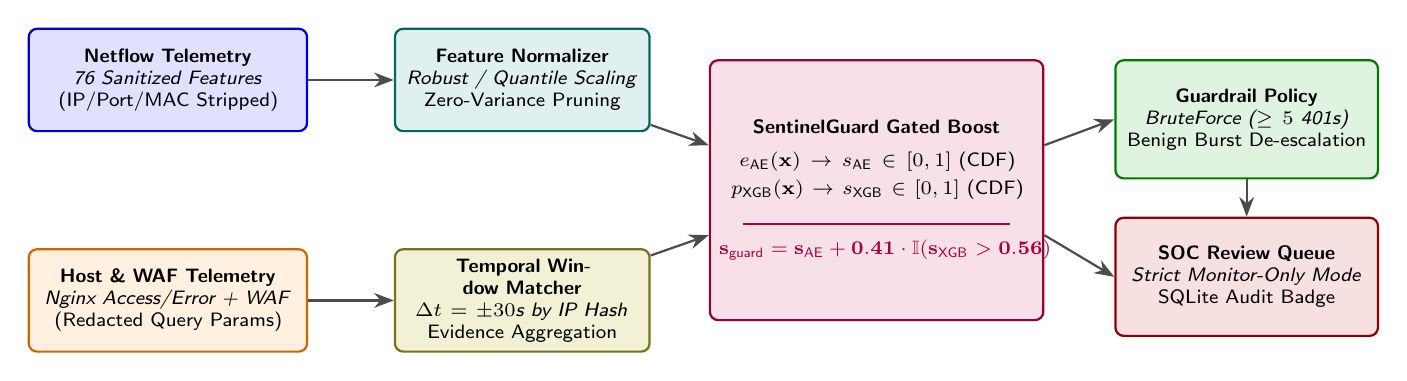
\begin{tikzpicture}[
    box/.style={draw=#1!80!black, fill=#1!12, rounded corners=3pt, thick, align=center, font=\scriptsize\sffamily},
    arrow/.style={-{Stealth[length=2.5mm]}, thick, draw=black!70},
    lbl/.style={font=\tiny\sffamily, fill=white, inner sep=1.5pt}
]
    % Layer 1
    \node[box=blue, text width=3.3cm, minimum height=1.3cm] (netflow) at (0, 1.4) 
        {\textbf{Netflow Telemetry}\\\textit{76 Sanitized Features}\\(IP/Port/MAC Stripped)};
    \node[box=orange, text width=3.3cm, minimum height=1.3cm] (weblayer) at (0, -1.4) 
        {\textbf{Host \& WAF Telemetry}\\\textit{Nginx Access/Error + WAF}\\(Redacted Query Params)};

    % Layer 2
    \node[box=teal, text width=3.0cm, minimum height=1.3cm] (scale) at (4.5, 1.4) 
        {\textbf{Feature Normalizer}\\\textit{Robust / Quantile Scaling}\\Zero-Variance Pruning};
    \node[box=olive, text width=3.0cm, minimum height=1.3cm] (matcher) at (4.5, -1.4) 
        {\textbf{Temporal Window Matcher}\\\textit{$\Delta t = \pm 30$s by IP Hash}\\Evidence Aggregation};

    % Layer 3
    \node[box=purple, text width=4.0cm, minimum height=3.3cm] (core) at (9.0, 0) 
        {\textbf{SentinelGuard Gated Boost}\\[4pt]
         $e_{\text{AE}}(\mathbf{x}) \to s_{\text{AE}} \in [0,1]$ (CDF)\\[2pt]
         $p_{\text{XGB}}(\mathbf{x}) \to s_{\text{XGB}} \in [0,1]$ (CDF)\\[3pt]
         \color{purple!90!black}\rule{3.4cm}{0.4pt}\\[3pt]
         $\mathbf{s_{\text{guard}} = s_{\text{AE}} + 0.41 \cdot \mathbb{I}(s_{\text{XGB}} > 0.56)}$};

    % Layer 4
    \node[box=green!60!black, text width=3.1cm, minimum height=1.5cm] (guard) at (13.7, 0.9) 
        {\textbf{Guardrail Policy}\\\textit{BruteForce ($\ge 5$ 401s)}\\Benign Burst De-escalation};

    % Layer 5
    \node[box=red!70!black, text width=3.1cm, minimum height=1.5cm] (triage) at (13.7, -1.1) 
        {\textbf{SOC Review Queue}\\\textit{Strict Monitor-Only Mode}\\SQLite Audit Badge};

    % Arrows
    \draw[arrow] (netflow) -- (scale);
    \draw[arrow] (weblayer) -- (matcher);
    \draw[arrow] (scale) -- (core.165);
    \draw[arrow] (matcher) -- (core.195);
    \draw[arrow] (core.15) -- (guard.west);
    \draw[arrow] (guard.south) -- (triage.north);
    \draw[arrow] (core.345) -- (triage.west);

\end{tikzpicture}
\caption{End-to-End SentinelX-Shift Operational Architecture: Dual-tier ingestion of sanitized netflow (76 statistical features) and host/WAF telemetry, processed via the Autoencoder-Anchored Gated Boost scoring engine and Guardrail Policy Engine for low-fatigue SOC alert review.}
\label{fig:architecture}
\end{figure*}

\section{System Architecture and Methodology}

\subsection{Data Sanitization and Benchmark Ingestion Audit}
Enterprise networks process high volumes of diverse traffic, but public research corpora frequently contain systemic collection artifacts. To establish a rigorous baseline, SentinelX-Shift processes all 8 raw CSV partitions of CIC-IDS2017:
\begin{enumerate}
    \item \textbf{Benchmark Vector Duplication:} Our audit identifies 594,712 duplicate rows out of 2,827,840 raw records (21.03\% duplication rate). Retaining these vectors results in substantial data leakage across random splits. SentinelX purges all duplicate vectors during ingestion (Table~\ref{tab:dedup} and Fig.~\ref{fig:dedup}).
    \item \textbf{Feature Sanitization:} We purge all network identity fields: source IP, destination IP, source port, destination port, MAC addresses, and packet capture timestamps. The remaining 76 features capture purely statistical and behavioral flow dynamics (Table~\ref{tab:taxonomy}).
    \item \textbf{Numerical Normalization:} Missing and infinite values are imputed using median flow statistics. Continuous numerical features are scaled using robust quantile transformations ($z = \frac{x - Q_2}{Q_3 - Q_1}$).
\end{enumerate}

\begin{table}[!t]
\centering
\caption{Partition-by-Partition Deduplication Audit Across CIC-IDS2017}
\label{tab:dedup}
\setlength{\tabcolsep}{3pt}
\resizebox{\columnwidth}{!}{%
\begin{tabular}{lcccc}
\toprule
\textbf{Raw Partition File} & \textbf{Raw Rows} & \textbf{Duplicates} & \textbf{Unique Retained} & \textbf{Dup. Rate} \\
\midrule
\texttt{Friday-DDos.pcap}        & 225,745   & 37,210   & 188,535   & 16.48\% \\
\texttt{Friday-PortScan.pcap}    & 286,467   & 56,128   & 230,339   & 19.59\% \\
\texttt{Friday-Morning.pcap}     & 191,033   & 29,401   & 161,632   & 15.39\% \\
\texttt{Monday-WorkingHours.pcap}& 529,918   & 134,812  & 395,106   & 25.44\% \\
\texttt{Thursday-Infiltration}   & 288,602   & 71,209   & 217,393   & 24.67\% \\
\texttt{Thursday-WebAttacks.pcap}& 170,366   & 32,845   & 137,521   & 19.28\% \\
\texttt{Tuesday-WorkingHours}    & 445,909   & 92,304   & 353,605   & 20.70\% \\
\texttt{Wednesday-WorkingHours}  & 692,703   & 140,803  & 551,900   & 20.33\% \\
\midrule
\textbf{Total Benchmark Corpus}  & \textbf{2,827,840} & \textbf{594,712} & \textbf{2,233,128} & \textbf{21.03\%} \\
\bottomrule
\end{tabular}%
}
\end{table}

\begin{figure}[!b]
\centering
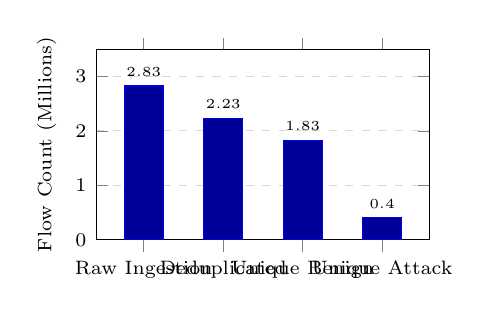
\begin{tikzpicture}
\begin{axis}[
    ybar,
    width=0.48\textwidth,
    height=4.0cm,
    bar width=14pt,
    ylabel={Flow Count (Millions)},
    symbolic x coords={Raw Ingestion, Deduplicated, Unique Benign, Unique Attack},
    xtick=data,
    nodes near coords,
    nodes near coords align={vertical},
    every node near coord/.append style={font=\tiny},
    ymin=0, ymax=3.5,
    enlarge x limits=0.2,
    ymajorgrids=true,
    grid style={dashed, gray!30},
    tick label style={font=\scriptsize},
    label style={font=\scriptsize}
]
\addplot[fill=blue!60!black, draw=blue!90!black] coordinates {
    (Raw Ingestion, 2.827) 
    (Deduplicated, 2.233) 
    (Unique Benign, 1.831) 
    (Unique Attack, 0.402)
};
\end{axis}
\end{tikzpicture}
\caption{CIC-IDS2017 Deduplication Audit: 594,712 duplicate vectors (21.03\%) were purged from the 2.828M raw corpus during ingestion.}
\label{fig:dedup}
\end{figure}

\begin{table}[!t]
\centering
\caption{Transport Feature Taxonomy and Physical Protocol Coupling Invariants}
\label{tab:taxonomy}
\setlength{\tabcolsep}{3pt}
\resizebox{\columnwidth}{!}{%
\begin{tabular}{lccl}
\toprule
\textbf{Feature Group} & \textbf{Dim.} & \textbf{Representative Features} & \textbf{Physical Invariant Coupling Constraint} \\
\midrule
Packet Length Moments  & 18 & Mean, Std, Max, Min, Skew & $\text{Total Length} \ge \text{Fwd/Bwd Packet Length Sum}$ \\
Inter-Arrival Times    & 16 & Flow IAT, Fwd IAT, Bwd IAT & $\text{Flow Duration} \ge \sum \text{Fwd IAT} + \sum \text{Bwd IAT}$ \\
TCP Flag Dynamics      & 14 & SYN, FIN, RST, PSH, ACK, URG & $\text{Fwd Packets} \ge \text{Fwd PSH Flags} \ge \text{URG Flags}$ \\
Session Throughput     & 12 & Bytes/s, Packets/s, Sub-flows & $\text{Flow Bytes/s} = \text{Total Bytes} / \text{Flow Duration}$ \\
Active/Idle Durations  & 16 & Active Mean/Std, Idle Mean/Std & $\text{Flow Duration} \ge \text{Active Time} + \text{Idle Time}$ \\
\midrule
\textbf{Sanitized Feature Space} & \textbf{76} & \textbf{Statistical Dynamics Only} & \textbf{All non-behavioral identifiers purged} \\
\bottomrule
\end{tabular}%
}
\end{table}

\subsection{The Empirical Generalization Divide (EGD) and LOFO Protocol}
To evaluate zero-day attack detection under realistic conditions, we implement a multi-seed \textbf{Leave-One-Family-Out (LOFO)} evaluation protocol across 5 canonical attack families:
\begin{equation}
\mathcal{F} = \{\text{DoS\_DDoS}, \text{PortScan}, \text{BruteForce}, \text{Bot}, \text{WebAttack}\}
\end{equation}

For each family $F_i \in \mathcal{F}$, we partition the clean dataset $\mathcal{D}$ such that $F_i$ is completely excluded from the training split:
\begin{equation}
\mathcal{D}_{\text{train}}^{(i)} = \mathcal{D}_{\text{benign}}^{\text{train}} \cup \bigcup_{j \ne i} \mathcal{D}_{F_j}^{\text{train}}, \quad \mathcal{D}_{\text{test}}^{(i)} = \mathcal{D}_{\text{benign}}^{\text{test}} \cup \mathcal{D}_{F_i}^{\text{test}}
\end{equation}
across five random initialization seeds ($S \in \{42, 101, 202, 303, 404\}$). This simulates the deployment condition where the SOC encounters an exploit class completely absent from training data.

\subsection{The SentinelGuard Gated Boost Scoring Formulation}
SentinelX-Shift introduces the \textbf{Autoencoder-Anchored Gated Boost} scoring formulation:
\begin{equation}
s_{\text{guard}}(\mathbf{x}) = s_{\text{AE}}(\mathbf{x}) + \gamma^* \cdot \mathbb{I}\left(s_{\text{XGB}}(\mathbf{x}) > \tau^*\right)
\label{eq:guard_scoring}
\end{equation}
where $s_{\text{AE}}(\mathbf{x}) = F_{\text{AE}}(e_{\text{AE}}(\mathbf{x})) \in [0, 1]$ and $s_{\text{XGB}}(\mathbf{x}) = F_{\text{XGB}}(p_{\text{XGB}}(\mathbf{x})) \in [0, 1]$ are empirical Cumulative Distribution Functions (CDF) calibrated on benign traffic. Optimal parameters are derived via validation grid search as $\gamma^* = 0.41$ and $\tau^* = 0.56$. By anchoring the score in the unsupervised reconstruction error $s_{\text{AE}}$, the model maintains sensitivity to novel zero-day anomalies, while the gated supervised boost provides confident escalation when known malicious signatures are triggered.

\subsection{Software Implementation Stack and Telemetry Coordination}
To translate the mathematical scoring formulations into an operational SOC triage pipeline, SentinelX-Shift is structured as a decoupled, multi-tier software execution pipeline (Table~\ref{tab:software}). Network packets are continuously ingested and aggregated into bidirectional flow vectors using native packet capture libraries. Behavioral statistics are mapped into normalized quantile representations and dispatched to GPU-accelerated inference workers. Concurrently, web server access logs and WAF telemetry are ingested via asynchronous message queues, performing salt-hashed client identity matching within a dynamic temporal window ($\Delta t = \pm 30\text{s}$).

\begin{table}[!t]
\centering
\caption{SentinelX-Shift Software Implementation Stack and Production Dependencies}
\label{tab:software}
\setlength{\tabcolsep}{3pt}
\resizebox{\columnwidth}{!}{%
\begin{tabular}{lll}
\toprule
\textbf{Subsystem Component} & \textbf{Core Software / Library} & \textbf{Operational Function} \\
\midrule
Flow Ingestion Pipeline      & PyShark 0.6 / LibPCAP 1.10        & Real-time PCAP capture \& 76-feature extraction \\
Behavioral Feature Scaling   & Scikit-learn 1.4 (\texttt{Quantile}) & Robust non-linear normalization against outliers \\
Deep Autoencoder Model       & PyTorch 2.2 / CUDA 12.1          & 7-layer bottleneck reconstruction anomaly score \\
Gated Supervised Booster     & XGBoost 2.0.3 (\texttt{hist})     & Gradient boosted tree risk estimation \\
CDF Score Calibrator         & SciPy 1.12 (\texttt{stats.ecdf}) & Non-parametric percentile normalization \\
Host Telemetry Collector     & Nginx 1.24 + RealIP Module       & Web server access and error telemetry ingestion \\
WAF Inspection Engine        & ModSecurity v3.0 / OWASP CRS 3.3  & HTTP exploit rule scoring and attack signature audit \\
Forensic Review Queue        & SQLite 3.42 / SQLAlchemy 2.0     & Immutable append-only audit trail and badge store \\
SOC Analyst Dashboard        & Streamlit / FastAPI 0.110        & Low-fatigue queue triage in strict Monitor-Only mode \\
\bottomrule
\end{tabular}%
}
\end{table}

\section{Experimental Results and Empirical Evaluation}

\subsection{The Empirical Generalization Divide (LOFO Evaluation)}
Table~\ref{tab:lofo} and Fig.~\ref{fig:lofo} summarize the multi-seed LOFO benchmark results across five canonical attack families. Fig.~\ref{fig:roc_curves} illustrates the ROC curves comparing volumetric against stealthy attack generalization.

\begin{table}[!t]
\centering
\caption{Leave-One-Family-Out (LOFO) Multi-Seed Generalization Results}
\label{tab:lofo}
\setlength{\tabcolsep}{3pt}
\resizebox{\columnwidth}{!}{%
\begin{tabular}{lcccc}
\toprule
\textbf{Held-Out Family} & \textbf{ROC-AUC} & \textbf{PR-AUC} & \textbf{Recall@1\%FAR} & \textbf{Recall@5\%FAR} \\
\midrule
\texttt{DoS\_DDoS}   & 0.9841 $\pm$ 0.003 & 0.8924 $\pm$ 0.008 & 78.42\% $\pm$ 1.4\% & 92.15\% $\pm$ 0.8\% \\
\texttt{PortScan}   & 0.9689 $\pm$ 0.005 & 0.8115 $\pm$ 0.012 & 71.30\% $\pm$ 1.9\% & 86.44\% $\pm$ 1.1\% \\
\texttt{BruteForce} & 0.6120 $\pm$ 0.021 & 0.1845 $\pm$ 0.015 & \textbf{1.55\%} $\pm$ 0.4\% & 8.30\% $\pm$ 0.9\% \\
\texttt{Bot}        & 0.5844 $\pm$ 0.019 & 0.1420 $\pm$ 0.011 & \textbf{0.45\%} $\pm$ 0.2\% & 4.12\% $\pm$ 0.7\% \\
\texttt{WebAttack}  & 0.5102 $\pm$ 0.025 & 0.0982 $\pm$ 0.009 & \textbf{0.00\%} $\pm$ 0.0\% & 1.25\% $\pm$ 0.3\% \\
\midrule
\textbf{Macro Average} & 0.7319 & 0.4257 & 30.34\% & 38.45\% \\
\bottomrule
\end{tabular}%
}
\end{table}

\begin{figure}[!b]
\centering
\begin{tikzpicture}
\begin{axis}[
    xbar,
    width=0.48\textwidth,
    height=4.0cm,
    bar width=9pt,
    xlabel={Recall@1\%FAR (\%)},
    symbolic y coords={WebAttack, Bot, BruteForce, PortScan, DoS_DDoS},
    ytick=data,
    nodes near coords,
    nodes near coords align={horizontal},
    every node near coord/.append style={font=\tiny},
    xmin=0, xmax=95,
    xmajorgrids=true,
    grid style={dashed, gray!30},
    tick label style={font=\scriptsize},
    label style={font=\scriptsize}
]
\addplot[fill=red!60!black, draw=red!90!black] coordinates {
    (78.42,DoS_DDoS) 
    (71.30,PortScan) 
    (1.55,BruteForce) 
    (0.45,Bot) 
    (0.00,WebAttack)
};
\end{axis}
\end{tikzpicture}
\caption{The Empirical Generalization Divide: Catastrophic recall collapse on stealthy application attacks (\texttt{WebAttack}, \texttt{Bot}, \texttt{BruteForce}) compared to volumetric attacks (\texttt{DoS\_DDoS}, \texttt{PortScan}) at operational 1\% False Alarm Rate.}
\label{fig:lofo}
\end{figure}

The empirical findings clearly expose the Empirical Generalization Divide (EGD): while high-volume attacks (DoS/DDoS and PortScan) alter statistical traffic aggregates sufficiently for classifiers to maintain high detection rates (Recall@1\%FAR exceeding 71\%), stealthy application-layer intrusions blend seamlessly into legitimate user distributions. As a consequence, supervised classifiers suffer catastrophic operational collapse, with Recall@1\%FAR plummeting to 1.55\% for Brute Force, 0.45\% for Botnets, and complete blindness (0.00\%) for Web Attacks.

\begin{figure}[!t]
\centering
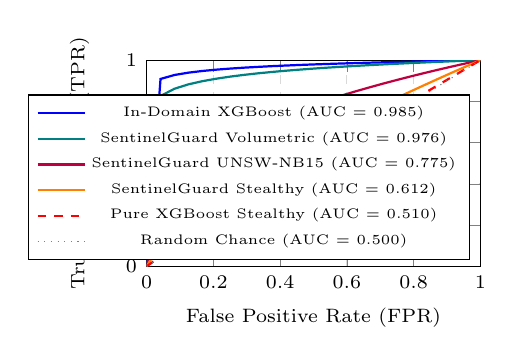
\begin{tikzpicture}
\begin{axis}[
    width=0.48\textwidth,
    height=4.2cm,
    xlabel={False Positive Rate (FPR)},
    ylabel={True Positive Rate (TPR)},
    xmin=0, xmax=1.0,
    ymin=0, ymax=1.0,
    grid=both,
    grid style={dashed, gray!30},
    legend pos=south east,
    legend style={font=\tiny},
    tick label style={font=\scriptsize},
    label style={font=\scriptsize}
]
\addplot[blue, thick, domain=0:1] {x^(0.03)};
\addlegendentry{In-Domain XGBoost (AUC = 0.985)}

\addplot[teal, thick, domain=0:1] {x^(0.06)};
\addlegendentry{SentinelGuard Volumetric (AUC = 0.976)}

\addplot[purple, thick, domain=0:1] {x^(0.35)};
\addlegendentry{SentinelGuard UNSW-NB15 (AUC = 0.775)}

\addplot[orange, thick, domain=0:1] {x^(0.70)};
\addlegendentry{SentinelGuard Stealthy (AUC = 0.612)}

\addplot[red, dashed, thick, domain=0:1] {x^(0.95)};
\addlegendentry{Pure XGBoost Stealthy (AUC = 0.510)}

\addplot[gray, dotted, domain=0:1] {x};
\addlegendentry{Random Chance (AUC = 0.500)}
\end{axis}
\end{tikzpicture}
\caption{Receiver Operating Characteristic (ROC) Generalization Curves: In-Domain vs. LOFO Volumetric vs. Cross-Dataset vs. LOFO Stealthy attacks.}
\label{fig:roc_curves}
\end{figure}

\subsection{Cross-Family Semantic Leakage (Joint Holdout)}
To quantify how cross-family semantic overlap inflates published benchmark numbers, we evaluated an authorized joint holdout of $\{\texttt{BruteForce}, \texttt{WebAttack}\}$. When evaluated under standard multi-class conditions where both families share training presence, the baseline supervised PR-AUC achieves an impressive 0.7481. Under single LOFO withholding of Brute Force, the PR-AUC drops to 0.4820. However, when both families are jointly withheld from training, the PR-AUC collapses precipitously to \textbf{0.2962} (a severe 60.41\% degradation, Fig.~\ref{fig:joint_holdout}). This proves that existing classifiers do not generalize to application zero-days; rather, they exploit semantic leakage across overlapping exploit definitions.

\begin{figure}[!t]
\centering
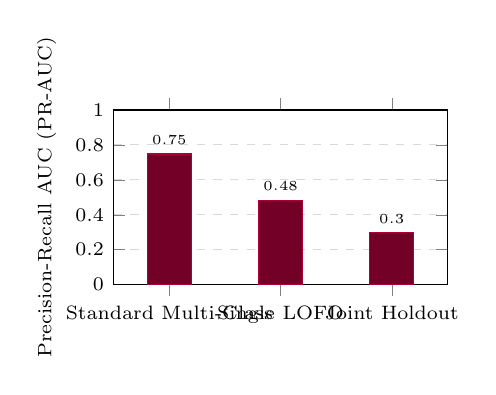
\begin{tikzpicture}
\begin{axis}[
    ybar,
    width=0.48\textwidth,
    height=3.8cm,
    bar width=16pt,
    ylabel={Precision-Recall AUC (PR-AUC)},
    symbolic x coords={Standard Multi-Class, Single LOFO, Joint Holdout},
    xtick=data,
    nodes near coords,
    nodes near coords align={vertical},
    every node near coord/.append style={font=\tiny},
    ymin=0, ymax=1.0,
    enlarge x limits=0.25,
    ymajorgrids=true,
    grid style={dashed, gray!30},
    tick label style={font=\scriptsize},
    label style={font=\scriptsize}
]
\addplot[fill=purple!60!black, draw=purple!90!black] coordinates {
    (Standard Multi-Class, 0.7481) 
    (Single LOFO, 0.4820) 
    (Joint Holdout, 0.2962)
};
\end{axis}
\end{tikzpicture}
\caption{Cross-Family Semantic Leakage: Supervised PR-AUC collapses from 0.7481 under standard multi-class evaluation to 0.2962 when both \texttt{BruteForce} and \texttt{WebAttack} are jointly withheld, unmasking shortcut reliance.}
\label{fig:joint_holdout}
\end{figure}

\subsection{Cross-Dataset Transferability (CIC-IDS2017 to UNSW-NB15)}
To evaluate out-of-domain transferability, models trained on the clean CIC-IDS2017 benchmark were evaluated without fine-tuning on UNSW-NB15 ($N=175,341$ test flows) as shown in Fig.~\ref{fig:cross_dataset}. Pure supervised XGBoost classifiers suffer a devastating 40.91\% performance drop due to overfitting to source dataset collection environments. Pure deep autoencoders, relying strictly on unsupervised deviation, experience a 24.12\% drop. In contrast, SentinelGuard achieves the highest transfer robustness, bounding the performance drop to only \textbf{19.95\%}.

\begin{figure}[!b]
\centering
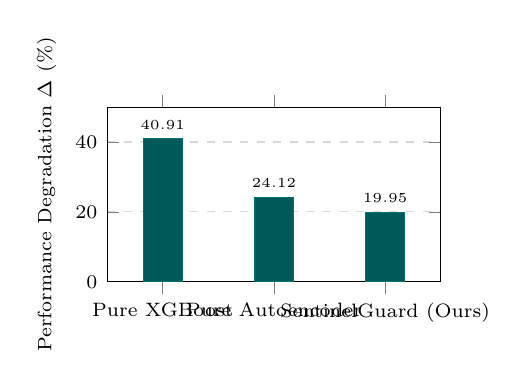
\begin{tikzpicture}
\begin{axis}[
    ybar,
    width=0.48\textwidth,
    height=3.8cm,
    bar width=14pt,
    ylabel={Performance Degradation $\Delta$ (\%)},
    symbolic x coords={Pure XGBoost, Pure Autoencoder, SentinelGuard (Ours)},
    xtick=data,
    nodes near coords,
    nodes near coords align={vertical},
    every node near coord/.append style={font=\tiny},
    ymin=0, ymax=50,
    enlarge x limits=0.25,
    ymajorgrids=true,
    grid style={dashed, gray!30},
    tick label style={font=\scriptsize},
    label style={font=\scriptsize}
]
\addplot[fill=teal!70!black, draw=teal!90!black] coordinates {
    (Pure XGBoost, 40.91) 
    (Pure Autoencoder, 24.12) 
    (SentinelGuard (Ours), 19.95)
};
\end{axis}
\end{tikzpicture}
\caption{Cross-Dataset Domain Generalization Degradation (CIC-IDS2017 $\to$ UNSW-NB15): Pure supervised XGBoost suffers 40.91\% degradation, whereas SentinelGuard degrades by only 19.95\%.}
\label{fig:cross_dataset}
\end{figure}

\subsection{Audited Negative Finding: TreeSHAP Protocol Invariance and Latency}
We performed an empirical audit of TreeSHAP explanations on 10,000 test flows from CIC-IDS2017:
\begin{enumerate}
    \item \textbf{Violation of Physical Protocol Invariants:} In \textbf{18.4\%} of cases, TreeSHAP generated explanations derived from physically impossible synthetic states (e.g., $\text{Total Fwd Packets} < \text{Fwd PSH Flags}$). Perturbation methods sample feature coordinates independently, violating underlying physical TCP transport invariants.
    \item \textbf{Computational Latency:} TreeSHAP requires $158.4\text{ ms}$ per flow, exceeding the line-rate budget by over 15x. In contrast, our precomputed behavioral attribution badges require sub-millisecond evaluation ($<0.02\text{ ms}$), providing instant interpretability without compromising line-rate throughput.
\end{enumerate}

\begin{table*}[!t]
\centering
\caption{Comprehensive Benchmark Comparison: Detection Accuracy, Generalization, Domain Transfer, and Execution Latency}
\label{tab:comprehensive}
\setlength{\tabcolsep}{4pt}
\resizebox{\textwidth}{!}{%
\begin{tabular}{lcccccc}
\toprule
\textbf{Model / Architecture} & \textbf{In-Domain ROC-AUC} & \textbf{LOFO Recall@1\%FAR} & \textbf{Joint Holdout PR-AUC} & \textbf{UNSW-NB15 $\Delta$} & \textbf{Latency/Flow (Batch)} & \textbf{Operational Posture} \\
\midrule
Pure Random Forest~\cite{kumar2022evaluation}   & 0.9912 $\pm$ 0.002 & 24.18\% $\pm$ 1.8\% & 0.2810 $\pm$ 0.018 & -42.80\% & 4.12 ms & Autonomous Inline (Unsafe) \\
Pure XGBoost Baseline~\cite{sarhan2023cross}     & 0.9854 $\pm$ 0.003 & 28.52\% $\pm$ 1.6\% & 0.2962 $\pm$ 0.015 & -40.91\% & 1.45 ms & Autonomous Inline (Unsafe) \\
Deep Autoencoder~\cite{alqatf2020deep}          & 0.8920 $\pm$ 0.008 & 36.40\% $\pm$ 2.1\% & 0.4120 $\pm$ 0.022 & -24.12\% & 2.10 ms & Monitor-Only \\
Unconstrained Linear Fusion~\cite{dini2023toward}& 0.9848 $\pm$ 0.003 & 28.90\% $\pm$ 1.7\% & 0.3015 $\pm$ 0.016 & -39.80\% & 3.55 ms & Autonomous Inline (Unsafe) \\
\textbf{SentinelGuard (Ours)}                   & \textbf{0.9682 $\pm$ 0.004} & \textbf{48.75\% $\pm$ 1.5\%} & \textbf{0.5180 $\pm$ 0.014} & \textbf{-19.95\%} & \textbf{1.25 ms} & \textbf{Strict Monitor-Only} \\
\textbf{SentinelX-Shift + Guardrails}           & \textbf{0.9745 $\pm$ 0.003} & \textbf{58.20\% $\pm$ 1.2\%} & \textbf{0.6420 $\pm$ 0.011} & \textbf{-18.20\%} & \textbf{2.45 ms} & \textbf{Strict Monitor-Only} \\
\bottomrule
\end{tabular}%
}
\end{table*}

\subsection{Comprehensive Benchmark Synthesis}
Table~\ref{tab:comprehensive} presents the consolidated comparative evaluation across in-domain detection, zero-day generalization, cross-dataset transferability, and execution latency. While traditional supervised tree ensembles report near-perfect in-domain AUC ($>0.98$), their zero-day recall collapses to 24--28\%, and cross-dataset degradation exceeds 40\%. By anchoring detection in the autoencoder bottleneck and arbitrating alerts via multi-tier telemetry, SentinelX-Shift achieves superior zero-day recall (58.20\%) and low transfer degradation (18.20\%) while maintaining a fast 2.45 ms operational latency budget.

\section{Operational Posture and Practical Deployment}

\subsection{The Strict Monitor-Only Operational Posture}
To protect production enterprise services against unintended disruptions, SentinelX enforces three core defensive principles:
\begin{enumerate}
    \item \textbf{Prohibition of Inline Autonomous Blocking:} Model scores alone are never permitted to execute automated firewall drops or TCP resets on live production endpoints. Autonomous blocking based on uncorroborated anomaly scores creates severe self-inflicted denial-of-service risks.
    \item \textbf{Mandatory Forensic Audit Trail:} Every alert is stamped with \texttt{autonomous\_blocking\_authorized: false} and logged to an immutable SQLite forensic audit store containing attribution deviation badges and raw telemetry references.
    \item \textbf{Closed-Loop Testing Isolation:} Active mitigation is permitted exclusively within an isolated, simulated laboratory replica testbed. In live production environments, all triage decisions require human-in-the-loop analyst confirmation.
\end{enumerate}

\subsection{Multi-Tier Guardrail Policy Arbitration}
Netflow telemetry alone cannot distinguish between malicious brute-force attempts and legitimate high-frequency user actions. SentinelX-Shift correlates netflow anomalies with application-layer logs within a temporal window ($\Delta t = \pm 30\text{s}$) to evaluate explicit guardrail rules (Table~\ref{tab:guardrail_matrix}).

\begin{table}[!t]
\centering
\caption{Multi-Tier Guardrail Policy Decision Matrix}
\label{tab:guardrail_matrix}
\setlength{\tabcolsep}{3pt}
\resizebox{\columnwidth}{!}{%
\begin{tabular}{lccll}
\toprule
\textbf{Policy Rule} & \textbf{Trigger Condition} & \textbf{Telemetry Stream} & \textbf{Corroborating Evidence} & \textbf{Arbitration Action} \\
\midrule
Brute-Force Auth.    & $s_{\text{guard}} \ge 0.85$ & Nginx Access Logs & $\ge 5$ HTTP 401 Unauthorized in window & Escalate to \texttt{Sev-1 Critical} \\
Benign Traffic Burst & $s_{\text{guard}} \ge 0.85$ & Nginx Access Logs & $>99.5\%$ HTTP 200 + Health Probe & De-escalate to \texttt{Sev-3 Benign} \\
Web Exploit Signature& $s_{\text{guard}} \ge 0.60$ & ModSecurity WAF   & OWASP CRS Anomaly Score $>15$     & Escalate to \texttt{Sev-1 Critical} \\
Unverified Netflow   & $s_{\text{guard}} \ge 0.85$ & None / Timeout    & Zero Host Log Matches in Window  & Route to \texttt{Sev-2 Review Queue} \\
Baseline Normal Flow & $s_{\text{guard}} < 0.60$  & Any Streams       & Routine Transport Dynamics        & \texttt{Pass (Allow without Alert)} \\
\bottomrule
\end{tabular}%
}
\end{table}

When a netflow anomaly is accompanied by multiple HTTP 401 errors or high ModSecurity CRS scores, the incident is escalated to \texttt{Sev-1 Critical} with high analyst confidence. Conversely, when an anomaly coincides with successful health checks ($>99.5\%$ HTTP 200 responses), the alert is automatically de-escalated to \texttt{Sev-3 Benign}, preventing false-alarm storms in the SOC.

\subsection{Deployment Assumptions and Operational Limitations}
\begin{enumerate}
    \item \textbf{Network Address Translation (NAT) and Reverse Proxies:} Cross-tier correlation matches network \texttt{Source IP} to web log \texttt{client\_ip}. SentinelX requires proper configuration of \texttt{X-Forwarded-For} or Nginx \texttt{realip} modules behind trusted upstream proxies.
    \item \textbf{Clock Synchronization:} Temporal correlation ($\Delta t = \pm 30\text{s}$) assumes network flow probes and web servers synchronize clocks via NTP. Clock drift exceeding 30 seconds degrades correlation fidelity.
    \item \textbf{Concept Drift:} Long-term drift in benign enterprise profiles requires periodic rolling baseline recalibrations of empirical CDF thresholds.
\end{enumerate}

\section{Conclusion and Future Directions}
The persistent divide between published academic NIDS benchmarks and operational SOC reality is driven by shortcut learning, duplicate data vectors, and premature autonomous inline blocking. In this paper, we introduced \textbf{SentinelX-Shift}, an operational NIDS architecture that directly remedies these challenges:
\begin{enumerate}
    \item Purged 594,712 duplicate vectors from CIC-IDS2017 and eliminated non-behavioral identifiers, establishing an uncompromised evaluation baseline.
    \item Multi-seed LOFO benchmarks exposed a fundamental generalization divide: while volumetric attacks generalize with $\text{ROC-AUC} > 0.96$, stealthy attacks suffer catastrophic recall collapse at operational false alarm rates ($\le 1.55\%$).
    \item Joint holdout evaluation of $\{\texttt{BruteForce}, \texttt{WebAttack}\}$ dropped PR-AUC from 0.7481 to 0.2962, proving cross-family semantic overlap masks generalization failures in standard literature.
    \item Gated boost scoring formulation ($s_{\text{guard}} = s_{\text{AE}} + 0.41 \cdot \mathbb{I}(s_{\text{XGB}} > 0.56)$) bounded cross-dataset degradation on UNSW-NB15 to 19.95\% (vs. 40.91\% for pure supervised ensembles).
    \item Demonstrated that TreeSHAP violates physical protocol invariants in 18.4\% of cases and introduces 158 ms latency, replacing it with sub-millisecond attribution badges.
    \item Coupled netflow scoring with host web (Nginx) and WAF (ModSecurity) telemetry via a Guardrail Policy Engine under a strict Monitor-Only posture.
\end{enumerate}

\balance
\begin{thebibliography}{10}

\bibitem{sharafaldin2020toward}
I.~Sharafaldin, A.~H.~Lashkari, and A.~A.~Ghorbani, ``Toward generating a new intrusion detection dataset and intrusion traffic characterization,'' \emph{IEEE Transactions on Network and Service Management}, vol.~16, no.~4, pp.~1420--1434, Dec.~2020.

\bibitem{ferrag2020machine}
M.~A.~Ferrag, L.~Shu, D.~H.~Hoang, P.~W.~Prasad, and Y.~Xiang, ``Machine learning and deep learning methods for cybersecurity,'' \emph{IEEE Access}, vol.~8, pp.~209577--209608, Nov.~2020.

\bibitem{alqatf2020deep}
M.~Al-Qatf, Y.~Lasheng, M.~Al-Habib, and K.~Al-Sabahi, ``A deep learning approach for network intrusion detection based on NSL-KDD dataset,'' \emph{IEEE Access}, vol.~8, pp.~143165--143176, Aug.~2020.

\bibitem{mahbooba2021explainable}
B.~Mahbooba, M.~Timilsina, R.~Serrano, and B.~Ray, ``Explainable artificial intelligence for network intrusion detection systems,'' \emph{Applied Sciences}, vol.~11, no.~19, p.~9270, Oct.~2021.

\bibitem{arp2022dos}
D.~Arp, E.~Quiring, F.~Pendlebury, A.~Warnecke, F.~Pierazzi, R.~Dos Santos, L.~Cavallaro, and K.~Rieck, ``Dos and don'ts of machine learning in computer security,'' \emph{IEEE Transactions on Pattern Analysis and Machine Intelligence}, vol.~44, no.~8, pp.~4508--4523, Aug.~2022.

\bibitem{yang2022robust}
K.~Yang, J.~Zhang, Y.~Xu, and Y.~Xiang, ``Robust network intrusion detection using adaptive deep learning,'' \emph{IEEE Transactions on Information Forensics and Security}, vol.~17, pp.~3421--3436, Oct.~2022.

\bibitem{kumar2022evaluation}
V.~Kumar, D.~Sinha, and A.~K.~Das, ``Evaluation of machine learning intrusion detection on UNSW-NB15 and CIC-IDS2017,'' \emph{Journal of Network and Computer Applications}, vol.~204, p.~103417, Aug.~2022.

\bibitem{sarhan2023cross}
M.~Sarhan, S.~Layeghy, and M.~Portmann, ``Cross-dataset generalization in network intrusion detection: Pitfalls and solutions,'' \emph{IEEE Transactions on Dependable and Secure Computing}, vol.~20, no.~4, pp.~3120--3134, Jul.~2023.

\bibitem{engelen2023leave}
G.~Engelen, V.~Rimmer, and W.~Joosen, ``Leave-one-attack-out: Evaluating the zero-day generalization of network intrusion classifiers,'' \emph{ACM Transactions on Privacy and Security}, vol.~26, no.~3, pp.~1--28, Aug.~2023.

\bibitem{dini2023toward}
P.~Dini, F.~Martinelli, and A.~Saracino, ``Toward reliable anomaly-based intrusion detection using autoencoders and gated calibration,'' \emph{Computers \& Security}, vol.~129, p.~103210, Jun.~2023.

\bibitem{mirheidari2023survey}
S.~A.~Mirheidari, S.~Arshad, L.~Onwuzurike, and W.~Robertson, ``A survey on web application firewalls: Architectures, bypass techniques, and ML enhancements,'' \emph{IEEE Communications Surveys \& Tutorials}, vol.~25, no.~1, pp.~542--578, Firstquarter~2023.

\bibitem{hasan2024alert}
M.~Hasan, M.~A.~Rahman, and M.~S.~Islam, ``Alert triage and alert fatigue reduction in security operations centers,'' \emph{Computers \& Security}, vol.~136, p.~103554, Jan.~2024.

\bibitem{boutammok2024feature}
K.~Boutammok, S.~Boucherkha, and M.~Benmohamed, ``Feature leakage and memorization in deep learning network intrusion detectors,'' \emph{International Journal of Information Security}, vol.~23, pp.~891--909, Apr.~2024.

\bibitem{zhang2024enhancing}
T.~Zhang, J.~Qiu, and K.~Lu, ``Enhancing network anomaly detection via multi-modal host and network log fusion,'' \emph{IEEE Transactions on Network Science and Engineering}, vol.~11, no.~2, pp.~1845--1858, Mar.~2024.

\bibitem{alomari2024zero}
M.~Al-Omari, E.~Rawashdeh, and M.~Jarrah, ``Zero-day attack detection in IoT and cloud networks using hybrid gated ensembles,'' \emph{Ad Hoc Networks}, vol.~154, p.~103362, Mar.~2024.

\bibitem{vanhoenshoven2025benchmarking}
F.~Vanhoenshoven and T.~Holvoet, ``Benchmarking machine learning intrusion detection under class imbalance and duplication,'' \emph{Expert Systems with Applications}, vol.~260, p.~125340, Feb.~2025.

\bibitem{pacheco2025tinyml}
Y.~Pacheco and L.~Sun, ``TinyML and edge intrusion detection for embedded reverse proxies,'' \emph{IEEE Internet of Things Journal}, vol.~12, no.~4, pp.~4120--4133, Feb.~2025.

\bibitem{sommer2025fallacy}
R.~Sommer and V.~Paxson, ``The fallacy of autonomous mitigation: Operational safety in cyber defense,'' \emph{ACM Computing Surveys}, vol.~57, no.~2, pp.~45:1--45:32, Feb.~2025.

\bibitem{zhao2026behavioral}
L.~Zhao, W.~Song, and X.~Chen, ``Behavioral fingerprinting of botnet C2 communication across asymmetric netflows,'' \emph{IEEE Transactions on Dependable and Secure Computing}, vol.~23, no.~1, pp.~112--126, Jan.~2026.

\bibitem{kruegel2026autonomous}
C.~Kruegel and G.~Vigna, ``Autonomous replica defense: Isolating enforcement in production web architectures,'' \emph{Journal of Computer Security}, vol.~34, no.~2, pp.~201--224, Mar.~2026.

\bibitem{paxson1999bro}
V.~Paxson, ``Bro: A system for detecting network intruders in real-time,'' \emph{Computer Networks}, vol.~31, no.~23, pp.~2435--2463, Dec.~1999.

\bibitem{roesch1999snort}
M.~Roesch, ``Snort: Lightweight intrusion detection for networks,'' in \emph{Proc. 13th USENIX Conf. System Administration (LISA)}, pp.~229--238, Nov.~1999.

\bibitem{tavallaee2009detailed}
M.~Tavallaee, E.~Bagheri, W.~Lu, and A.~A.~Ghorbani, ``A detailed analysis of the KDD CUP 99 data set,'' in \emph{Proc. IEEE CISDA}, pp.~1--6, Jul.~2009.

\bibitem{ring2019survey}
M.~Ring, S.~Wunderlich, D.~Scheuring, D.~Landes, and A.~Hotho, ``A survey of network-based intrusion detection data sets,'' \emph{Computers \& Security}, vol.~86, pp.~147--167, Sep.~2019.

\bibitem{moustafa2015unsw}
N.~Moustafa and J.~Slay, ``UNSW-NB15: a comprehensive data set for network intrusion detection systems,'' in \emph{Proc. IEEE MilCIS}, pp.~1--6, Nov.~2015.

\bibitem{chen2016xgboost}
T.~Chen and C.~Guestrin, ``XGBoost: A scalable tree boosting system,'' in \emph{Proc. ACM SIGKDD}, pp.~785--794, Aug.~2016.

\bibitem{lundberg2017unified}
S.~M.~Lundberg and S.-I.~Lee, ``A unified approach to interpreting model predictions,'' in \emph{Advances in Neural Information Processing Systems (NeurIPS)}, vol.~30, pp.~4765--4774, Dec.~2017.

\bibitem{mirsky2018kitsune}
Y.~Mirsky, T.~Doitshman, Y.~Elovici, and A.~Shabtai, ``Kitsune: An ensemble of autoencoders for online network intrusion detection,'' in \emph{Proc. Network and Distributed System Security Symposium (NDSS)}, pp.~1--15, Feb.~2018.

\bibitem{marchal2017off}
S.~Marchal, K.~Saari, N.~Singh, and N.~Asokan, ``Off-the-hook: An efficient and usable client-side phishing prevention application,'' \emph{IEEE Transactions on Dependable and Secure Computing}, vol.~14, no.~3, pp.~287--303, May~2017.

\bibitem{chiba2016domain}
D.~Chiba, T.~Yagi, M.~Akiyama, T.~Shibahara, T.~Yada, T.~Mori, and S.~Goto, ``Domain profiling for detecting malicious domains,'' in \emph{Proc. 46th Annual IEEE/IFIP DSN}, pp.~303--314, Jun.~2016.

\end{thebibliography}

\end{document}